\documentclass[border=10pt]{standalone}

\usepackage{tikz}
\usepackage{tikzsymbols}
\usetikzlibrary{calc,patterns,shapes.geometric}

\def\centerarc[#1](#2)(#3:#4:#5){\draw[#1] ($(#2)+({#5*cos(#3)},{#5*sin(#3)})$) arc (#3:#4:#5);}

\begin{document}
	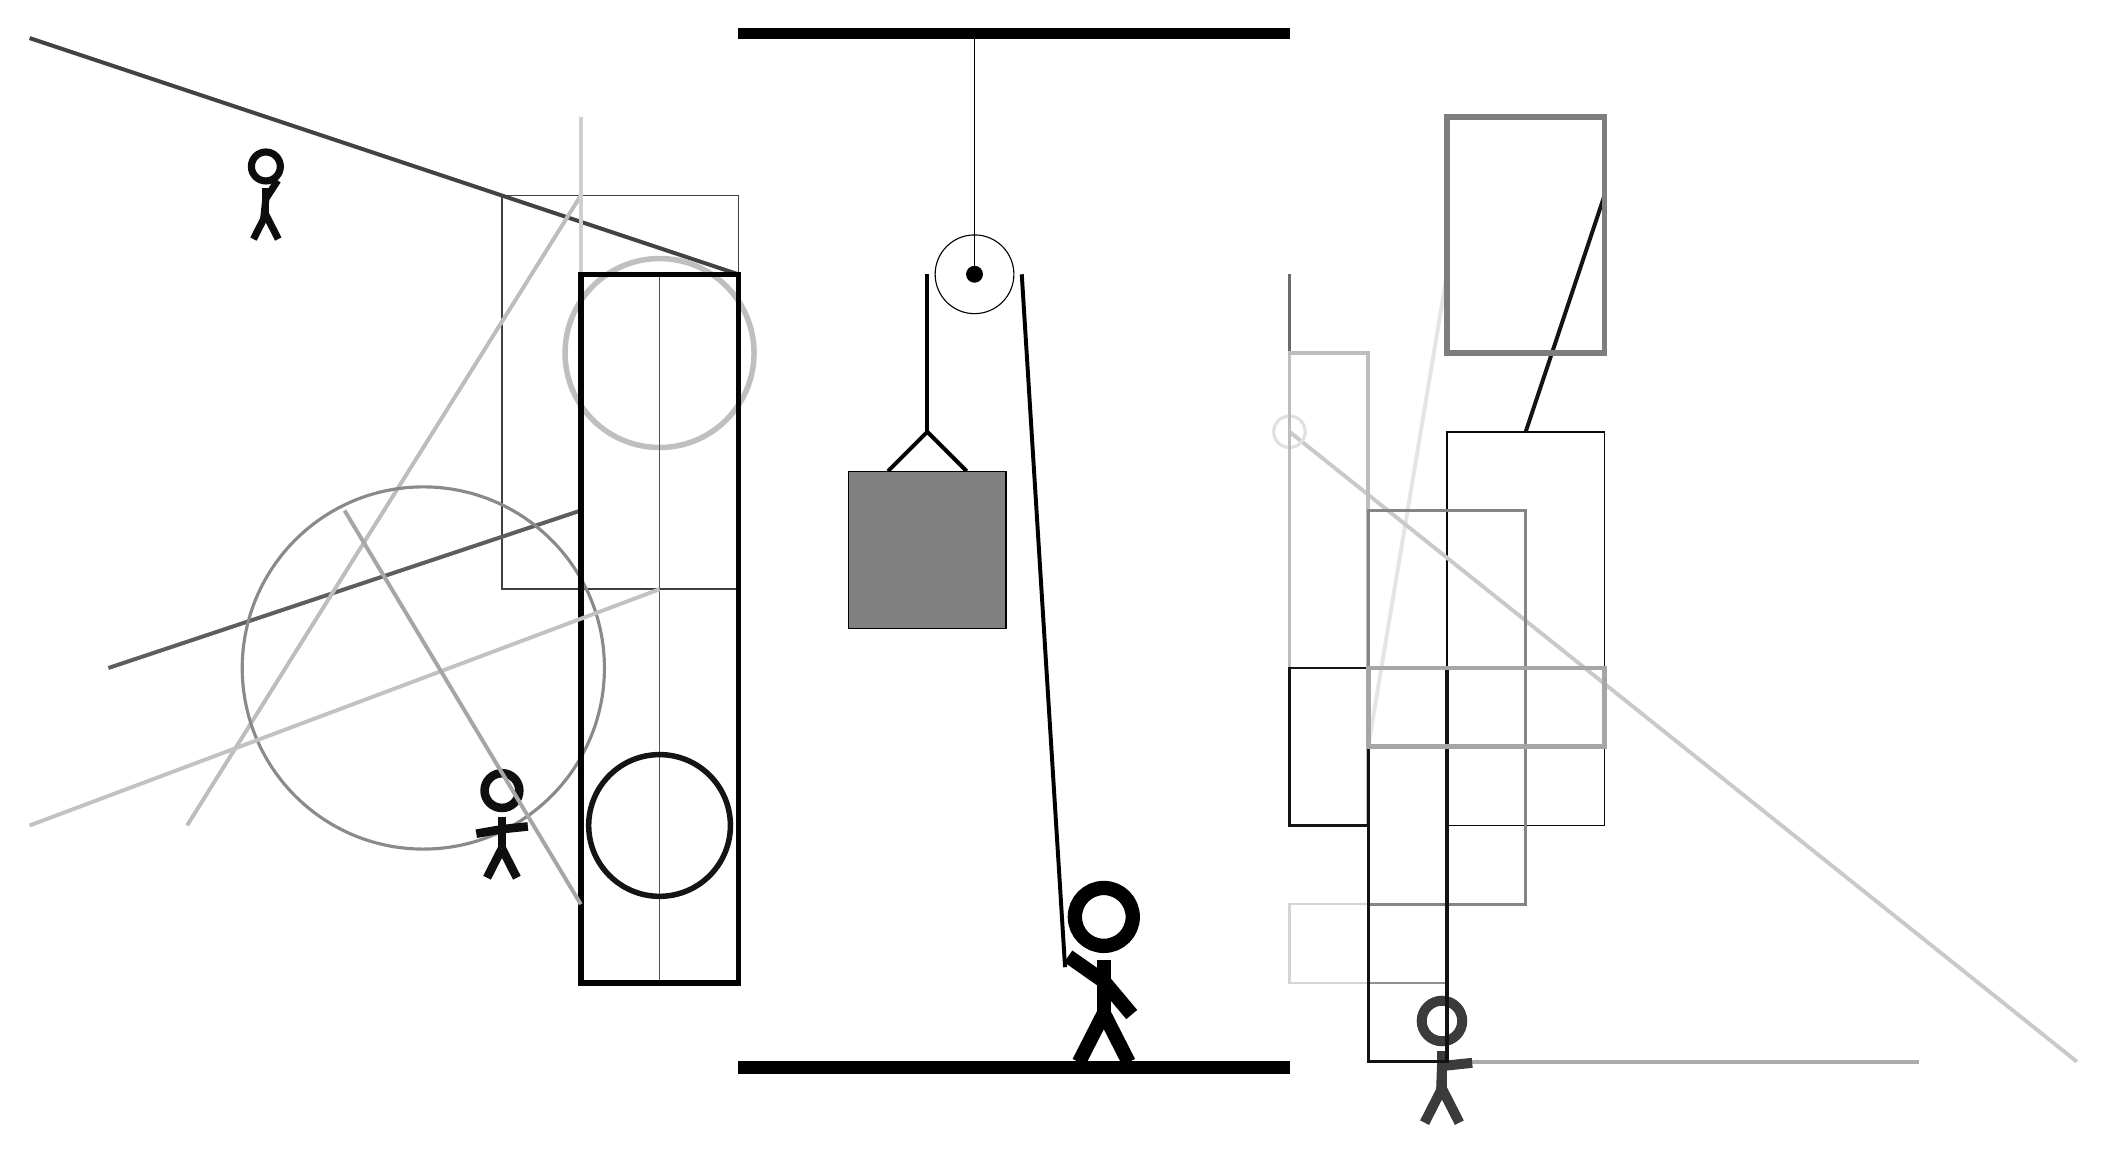
\begin{tikzpicture}
		%%%%% START %%%%%
		
		\draw[fill=black] (-2, 10) rectangle (5, 10.125);
		
		\draw (1, 7) circle (0.5);
		\draw[fill=black] (1, 7) circle (0.1);
		\draw (1, 10) -- (1, 7);
		
		\draw[line width=0.5mm] (-0.1, 4.5) -- (0.4, 5.0) -- (0.9, 4.5);
		\draw[fill=black!50] (-0.6, 4.5) rectangle (1.4, 2.5);
		
		\draw[line width=0.5mm] (0.4, 7) -- (0.4, 5.0);
		\centerarc[line width=0.5mm](1, 7)(0:180:0.6);
		\draw[line width=0.5mm](1.6, 7) -- (2.15, -1.8);
		
		\draw[line width=0.2mm, color=black!97] (7, 0) rectangle (9, 5);
		
		\draw[line width=0.2mm, color=black!75] (-2, 3) rectangle (-5, 8);
		\draw[line width=0.5mm, color=black!33](7, -3) -- (13, -3);
		\draw[line width=0.5mm, color=black!63](-4, 4) -- (-10, 2);
		\draw[line width=0.5mm, color=black!74](-2, 7) -- (-11, 10);
		\draw[line width=0.5mm, color=black!26](-4, 8) -- (-9, 0);
		\draw[line width=0.2mm, color=black!43] (6, -1) rectangle (7, -2);
		\node[line width=0.2mm, color=black!77] at (7, -3) {\Strichmaxerl[7][88][6]};
		\draw[line width=0.5mm, color=black!19] (-4, 9) rectangle (-4, -1);
		
		\draw [line width=0.4mm, color=black!46](-6, 2) circle (2.3);
		\draw[line width=0.3mm, color=black!17] (6, -1) rectangle (5, -2);
		\draw [line width=0.7mm, color=black!25](-3, 6) circle (1.2);
		\draw[line width=0.5mm, color=black!58](5, 7) -- (5, 1);
		\draw[line width=0.5mm, color=black!10](6, 1) -- (7, 7);
		\draw[line width=0.2mm, color=black!67] (-3, -2) rectangle (-4, 7);
		\node[line width=0.2mm, color=black!94] at (-5, 0) {\Strichmaxerl[6][10][6]};
		\draw [line width=0.7mm, color=black!92](-3, 0) circle (0.9);
		\draw[line width=0.5mm, color=black!92](9, 8) -- (8, 5);
		\draw[line width=0.7mm, color=black!99] (-4, -2) rectangle (-2, 7);
		\draw[line width=0.5mm, color=black!21](5, 5) -- (15, -3);
		\draw[line width=0.7mm, color=black!51] (7, 9) rectangle (9, 6);
		\draw [line width=0.4mm, color=black!12](5, 5) circle (0.2);
		\draw[line width=0.5mm, color=black!26] (6, 6) rectangle (5, 0);
		\node[line width=0.3mm, color=black!95] at (-8, 8) {\Strichmaxerl[5][84][57]};
		\draw[line width=0.3mm, color=black!92] (5, 0) rectangle (6, 2);
		\draw[line width=0.4mm, color=black!48] (6, 4) rectangle (8, -1);
		\draw[line width=0.4mm, color=black!93] (6, -3) rectangle (7, 2);
		\draw[line width=0.5mm, color=black!24](-3, 3) -- (-11, 0);
		\draw[line width=0.5mm, color=black!35](-7, 4) -- (-4, -1);
		\draw[line width=0.6mm, color=black!35] (6, 2) rectangle (9, 1);
		
		\node at (2.6, -1.9) {\Strichmaxerl[10][-35][-50]};
		
		\draw[fill=black] (-2, -3) rectangle (5, -3.15);
		
		%%%%% END %%%%%
	\end{tikzpicture}
\end{document}